% !TeX root = ../../thesis.tex
\chapter{背景知識}

\section{深層類神經網路(deep neural network)}

\subsection{簡介}

深層類神經網路(Deep Neural Network,DNN 或簡稱 NN)又稱「人工類神經網路(Artificial Neural Network,ANN)是來自於神經科學家麥氏(McCulloch)與皮氏(Mitts)等人在 1943 年提出 \cite{mcculloch1943logical},取法自生物神經連結的計算模型。以發展此類模型為主軸的心理學流派,在計算認知神經科學中被稱為「連結派(Connectionism)」,旨在模擬生物神經系統的連結,以模仿生物的各項功能。爾後在工程界進而透過機器學習的最佳化演算法,使得整個模型能夠藉由資料去貼合(Fit)理想的函數,以達成應用或工程上所需要的各種任務。因為該類網路的彈性與計算上易於平行化的特徵,能夠很恰當的利用諸如圖形處理器(Graphics Processing Unit,GPU)等硬體裝置的優勢,以求更好的描述資料分佈、達到前所未有的效能,因此近年在電腦科學的機器學習領域中獲得重大進展,現已成為人工智慧發展的主流。

深層類神經網路最基本的單位是「神經元(Neuron)」,模仿生物神經細胞接收訊號、處理到傳出的過程,每個神經元會接收一串數字作為輸入並計算出一個數字作為輸出,可用下列向量運算的式子描述:

$$y=\sigma(w^\top x + b) $$

其中 $x$ 是 $N$ 個輸入的數字,可描述為一個 $N$ 維的向量;$w$ 為該神經元對每個輸入值給予的權重,再對加權平均後的結果加上偏差值 $b$ 後,經過激發函數(Activation Function)$\sigma$ 的非線性轉換後最後得到輸出。其中常見的激發函數有線性整流單元(Rectified Linear Unit,ReLU)、S 函數(Sigmoid Function)或雙曲正切函數(Hyperbolic Tangent Function,$\tanh$)等等。

\begin{figure}

\centering

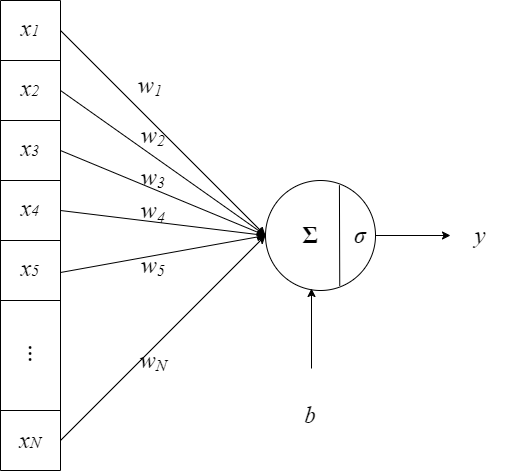
\includegraphics[width=0.5\linewidth]{figures/neuron.drawio.png}

\caption{神經元示意圖}

\label{fig:single-neuron}

\end{figure}

由多個神經元可形成單層感知機(Perceptron) \cite{rosenblatt1958perceptron},為了能夠處理更複雜的運算,多層感知機(Multi-layer Perceptron,MLP)被提出。透過梯度下降等演算法進行最佳化,以降低網路輸出與目標函數之間的誤差,再將此誤差藉由反向傳播演算法對整個網路的權重進行調整,以最好的擬合想要的函數。

\subsection{卷積式類神經網路}

 